% ---------------------------------------------------------------------------- %
\chapter{Desenvolvimento}
\label{cap:desenvolvimento}
% ---------------------------------------------------------------------------- %

\textit{PsyChO: The Ball} teve seu início em 2013 como \textit{PsyChObALL}. Durante os primeiros meses, o projeto servia como um meio prático de se aprender técnicas de programação e desenvolvimento de jogos e, aos poucos, foi tomando proporções maiores até ter seu primeiro lançamento em agosto de 2013. O jogo continuou em desenvolvimento até meados de 2014, mas lentamente começou a receber menos atualizações conforme seus criadores foram focando em outros projetos.

Foi somente no segundo semestre de 2015 que ele ressurgiu como \textit{PsyChO: The Ball}, na disciplina \textbf{MAC0214 - Atividade Curricular em Cultura e Extensão}. O objetivo do projeto era revitalizar o \textit{PsyChObALL} original, fazendo tudo do início e utilizando todo conhecimento acumulado durante a graduação. O fim de 2016 teve como resultado um protótipo bem elaborado do jogo, com todas mecânicas originais do \textit{PsyChObALL} implementadas e melhoradas.

O desenvolvimento do jogo passou por várias fases. Seguem neste capítulo algumas das infraestruturas mais importantes desenvolvidas para o projeto.

% ---------------------------------------------------------------------------- %
\section{STEAMING}
\label{sec:steaming}

Antes de começar o desenvolvimento direto de \textit{PsyChO: The Ball}, os primeiros meses foram direcionados em criar um template de jogos para o arcabouço \textit{Love2D}. Esse template se tornou o \textbf{STEAMING} (\textit{Simple TEmplAte for MakINg Games}) e todo o código do jogo foi construído em cima dele.

\textbf{STEAMING} possui duas características peculiares que foram vantajosas para o desenvolvimento do jogo: sua infraestrutura orientada a objetos para manipular elementos num jogo e sua estrutura para desenhar objetos na tela.

Todos os objetos no jogo foram herdados de uma classe básica chamada \textit{Element}. Um \textit{Element} pode possuir três atributos fundamentais: um tipo (chamado de \textit{type}), um subtipo (chamado de \textit{subtype}) e uma identificação única (chamada de \textit{id}). Com esses três atributos é possível agrupar, identificar, selecionar ou até mesmo destruir elementos no jogo com muita praticidade, ajudando imensamente seu desenvolvimento.

\textbf{STEAMING} reduz todo o \textit{pipeline gráfico} do jogo em camadas. Elementos do jogo desenháveis são atribuídos à alguma camada e a própria infraestrutura do template vai percorrer todas elas, em ordem, e desenhar os objetos dentro de cada uma, chamando o método correspondente da classe. Com essa organização é possível diagramar o \textit{design gráfico} do jogo bem mais facilmente e não se preocupar com objetos sendo desenhados na ordem certa. Entretanto, objetos na mesma camada são desenhados em uma ordem imprevisível, já que são armazenados dentro de uma \textit{tabela hash} sem ordem específica.

% ---------------------------------------------------------------------------- %
\section{Gerenciador de Saves}
\label{sec:gerenciador_de_saves}

Para armazenar dados entre partidas, foi desenvolvido um \textbf{gerenciador de saves}. Este é responsável por guardar as informações relevantes do jogo, como maiores pontuações, configurações de som escolhidas pelo usuário, se é a primeira vez que o jogador abriu o jogo, entre outras.

Todas as informações são guardadas em tabelas de Lua, que depois são transformadas no formato padronizado \textit{JSON} e salvas no disco rígido. Para recuperar essas informações, o \textbf{gerenciador de saves} faz a transformação inversa toda vez que o jogo é inicializado e atribui os valores para suas respectivas variáveis.

% ---------------------------------------------------------------------------- %
\section{Script de Fases}
\label{sec:level_script}

Para organizar o fluxo de eventos em cada nível do jogo, foi implementado um gerenciador de níveis. Assim foi possível abstrair a lógica de cada fase em \textit{scripts}.

Cada \textit{script} descreve em que sequência inimigos ou ações se desenrolam em cada nível do jogo. Isso facilitou imensamente no \textit{design} dos níveis, especialmente quando foi necessário balancear o jogo, pois o \textit{script} permite editar e visualizar facilmente cada nível em poucas linhas. Vários métodos foram criados para gerar padrões específicos de inimigos, dar vidas-extras para o Psycho ou até mesmo criar chefões.

Porém, para manter um ritmo durante o nível e não fazer o gerenciador rodar todas as linhas de uma vez, foi necessário usar corotinas. Elas permitem paralelizar o código e gerar múltiplos pontos de retorno para que o jogo aguarde certas condições antes de continuar o \textit{script} de um nível. Essas condições podem ser de tempo (como esperar 10 segundos antes de enviar a próxima sequência de inimigos) ou de aguardar até que não tenha um inimigo vivo na tela (utilizada, por exemplo, para esperar que o jogador destrua todos inimigos antes de avançar para o nível seguinte).

Para lidar com corotinas paradas, ou criar novas corotinas, vários métodos auxiliares foram implementados, sempre com o objetivo de abstrair o máximo possível para que mesmo um não-programador consiga criar seus próprios níveis no jogo.

% ---------------------------------------------------------------------------- %
\section{Shaders}
\label{sec:shaders}

Uma boa descrição de \textit{PsyChO: The Ball} seria: contém muitos círculos. Logo, como este é o elemento mais característico do jogo, é desejável que os círculos sejam visualmente agradáveis.

Inicialmente os círculos eram desenhados com os métodos imbutidos no arcabouço \textit{LÖVE}. Entretanto estes não utilizam nenhum algoritmo de suavização, como consequência as bordas dos círculos ficam serrilhadas e não combinam com a estética do jogo.

\begin{figure}[h!]

\includegraphics[scale=.3]{anti-aliasing}
\centering
\caption{Na esquerda um círculo sem anti-aliasing. Na direita um circulo com anti-aliasing.}
\end{figure}

Desta forma escrevemos um \textit{shader} que desenha círculos com bordas suavizadas (ou, como é conhecido esse efeito, \textit{anti-aliasing}). Utilizando a linguagem de \textit{shaders} da \textit{LÖVE} (muito semelhante à linguagem de \textit{shaders} do \textit{OpenGL}, \textit{GLSL}), um \textit{script} genérico consegue desenhar qualquer círculo com bordas suavizadas, dado o tamanho do seu diâmetro:

\begin{lstlisting}[language=java]
vec4 effect(vec4 color,Image text,vec2 text_coords,vec2 scrn_coords){
  vec4 pixel = Texel(text, text_coords); //This is the current pixel color
  vec2 center = vec2(0.5,0.5); //Center of the image
  pixel.a = 1 - smoothstep(.5 - 1/%f, .5, distance(center, text_coords));
  return pixel * color;
}
\end{lstlisting}

A primeira linha de nosso código define a função que criará o efeito desejado. Ela recebe como argumento a cor atual definida pela \textit{LÖVE}, a textura da imagem a ser desenhada, as coordenadas do atual pixel na imagem (normalizada no intervalo [0,1]) e as coordenadas do pixel em relação à tela. A segunda linha vai pegar a cor atual do pixel que estamos rodando a função,
enquanto a terceira linha define uma variável para representar o centro da imagem.

A linha 4 vai criar nosso efeito de anti-aliasing. Enviando o diâmetro do círculo para subsituir o \textit{\%f}, utilizamos a função \textit{smoothstep} que vai fazer interpolação da transparência em pixels que estão na borda de nosso círculo. Essa função vai retornar 0 caso o pixel esteja dentro do raio do círculo, e 1 caso esteja fora. Entretanto, se a posição estiver no intervalo de 1 pixel desse raio (e a distância de 1 pixel é determinada pela divisão 1/diâmetro do círculo, para receber o valor normalizado do mesmo), a função vai retornar um valor correspondente entre 0 e 1. Subtraindo de 1 o resultado teremos o valor de transparência (ou \textit{alpha}) de nosso pixel, assim chegando no resultado esperado.\\


Além disso, o jogo precisa de outro efeito realizado por \textit{shaders}: borrar a tela, denominado \textit{blur}. Esse efeito acontece quando o jogador pausa o jogo, de forma que somente a interface da tela de pausa fique nítida, enquanto todos outros elementos do jogo fiquem desfocados como se estivessem borrados.

\begin{figure}[h]
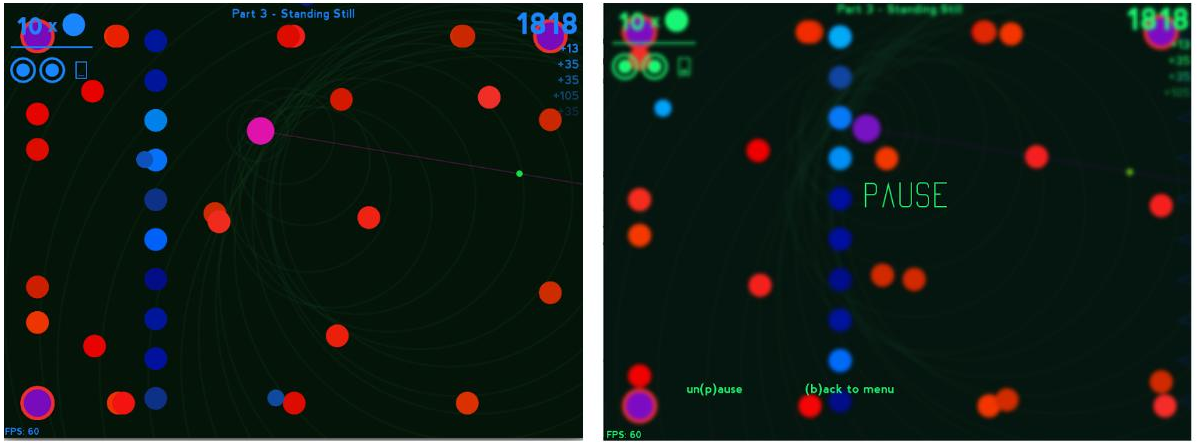
\includegraphics[scale=.5]{blur-ingame}
\centering
\caption{Na esquerda uma tela de jogo sem efeito de \textit{blur}. Na direita efeito de \textit{blur} aplicado.}
\end{figure}

Para atingir tal efeito foi criado dois \textit{scripts} de \textit{shader}, um que aplica um efeito de borrão horizontal e outro vertical. Assim, ao utilizar os dois em sequência, é possível chegar ao resultado esperado de uma tela desfocada, criando um efeito muito interessante enquanto o jogo estiver pausado.

\begin{lstlisting}[language=java]
  extern number win_width; //1 / (comprimento da tela)
  const float kernel[5] = float[](0.270270270, 0.1945945946, 0.1216216216,
                                  0.0540540541, 0.0162162162);
  vec4 effect(vec4 color, sampler2D tex, vec2 tex_coords, vec2 pos) {
    color = texture2D(tex, tex_coords) * kernel[0];
    for(int i = 1; i < 5; i++) {
      color += texture2D(tex,
            vec2(tex_coords.x + 6*i * win_width, tex_coords.y)) * kernel[i];
      color += texture2D(tex,
            vec2(tex_coords.x - 6*i * win_width, tex_coords.y)) * kernel[i];
    }
    return color;
  }
\end{lstlisting}

Acima podemos ver o código para o shader que cria o efeito de borrão horizontal. A parte interessante consiste nas linha 2-3 e o laço das linhas 9-14. Nas linhas 2 e 3 definimos nosso \textit{kernel}, um vetor de \textit{floats} que vai ser aplicado em nosso pixel. O laço começando na linha 9 vai somar ao pixel atual porcentagens das cores dos pixels à esquerda e à direita do pixel, criando uma média das cores ao redor (horizontalmente apenas). Aplicando em cada pixel temos parte do efeito desejado.

O código do \textit{shader} de desfocamento vertical é análogo ao horizontal, utilizando as cores acima e abaixo de cada pixel, e utilizando a altura da tela, em vez do comprimento para saber o tamanho vertical de um pixel:

\begin{lstlisting}[language=java]
extern number win_height; //1 / (altura da tela)
const float kernel[5] = float[](0.270270270, 0.1945945946, 0.1216216216,
                                0.0540540541, 0.0162162162);
vec4 effect(vec4 color, sampler2D tex, vec2 tex_coords, vec2 pos) {
  color = texture2D(tex, tex_coords) * kernel[0];
  for(int i = 1; i < 5; i++) {
    color += texture2D(tex,
          vec2(tex_coords.x, tex_coords.y + 6*i * win_height)) * kernel[i];
    color += texture2D(tex,
          vec2(tex_coords.x, tex_coords.y - 6*i * win_height)) * kernel[i];
  }
  return color;
}
\end{lstlisting}

Para aplicar os dois shaders na mesma imagem, utilizamos uma das ferramentas do arcabouço \textit{LOVE2D}: \textit{canvas}. Estes servem para definir telas intermediárias de renderização. Assim desenhamos primeiramente os elementos de interesse com o \textit{shader} horizontal em um canvas. Logo em seguida renderizamos esse canvas na janela principal do jogo, agora aplicando o \textit{vertical}, chegando no efeito desejado.

\begin{figure}[h!]
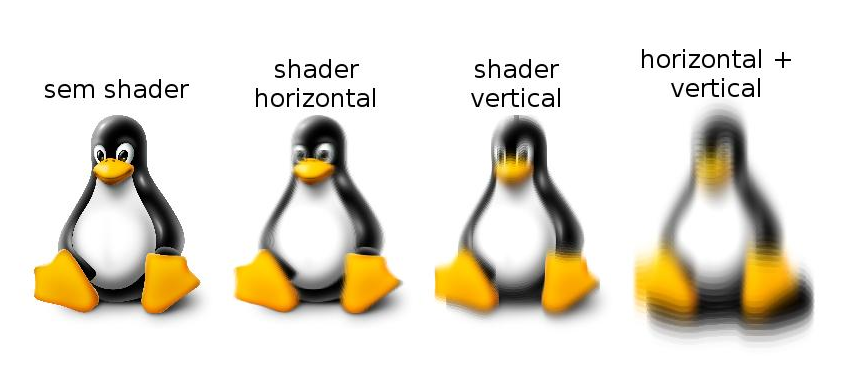
\includegraphics[scale=.4]{blur-effect}
\centering
\caption{Diferença visual da utilização e combinação dos \textit{shaders} para efeito \textit{blur}.}
\end{figure}


% ---------------------------------------------------------------------------- %
\section{Juiceness}
\label{sec:juiceness}

Além desses efeitos com \textit{shaders}, um grande foco no desenvolvimento do \textit{PsyChO: The Ball} foi em deixar o jogo mais \textit{juicy}. Isso é realizado com vários efeitos pequenos mas que tentam melhorar a experiência do jogador. \textit{Juicy} vem do termo \textit{Juiciness}, criado pelos desenvolvedores de jogos Martin Jonasson e Petri Purho, em uma palestra sobre \textit{Game Design}\cite{martinpetri}. Nela eles definem \textit{Juiciness} como uma recompensa ou fortalecimento de uma experiência, dada alguma ação do usuário e geralmente transmitida por efeitos especiais, tais como explosões, tremer a tela, ou até mesmo por efeitos sonoros.

Além disso, é considerado um efeito \textit{Juicy}, a utilização de interpolações e transições em vez de mudanças brutas de valores. Quase todas as transições do jogo são feitas desta forma. Um bom exemplo disso é a movimentação do personagem principal, \textit{Psycho}. Em vez dele ter uma velocidade constante quando se move, o Psycho tem uma leve aceleração quando começa seu movimento e uma leve desaceleração quando o jogador solta o comando de andar. Isso cria uma ilusão de movimento muito mais realista e agradável para o jogador em contraponto a uma velocidade que se inicia e acaba instantaneamente.

Outro efeito implementado no jogo, para aumentar a \textit{Juiciness}, é a explosão de partículas toda vez que um inimigo morre. Vários pequenos círculos de tamanho e velocidade variados explodem assim que um inimigo é destruído, dando mais emoção ao jogo e satisfação ao jogador.

Como último exemplo de efeito \textit{juicy}, \textit{PsyChO: The Ball} utiliza um clássico nos jogos de hoje em dia: tremer a tela quando o jogador morre. Este efeito, apesar de bem simples de se implementar (já que só é preciso transladar todos elementos na tela alguns pixels para a frente e para trás), gera um grande impacto e imersão ao jogador.

% ---------------------------------------------------------------------------- %
\section{Problemas e Desafios}
\label{sec:problemas_e_desafios}

Durante o desenvolvimento de \textit{PsyChO: The Ball} surgiram vários problemas e desafios. Para consertar \textit{bugs} ou otimizar o código foi necessário aprender a fundo a linguagem Lua, explorar bibliotecas disponíveis e até mesmo relembrar algoritmos aprendidos no curso.

Um dos desafios mais interessantes que surgiu foi a transição de cor dos objetos. Para manter o tema psicodélico, quase todos objetos ficam transitando entre valores de uma tabela de cores própria. Essa transição, porém, nunca parecia natural e orgânica já que apenas eram interpolados os valores \textit{RGB} de um objeto para os valores alvo, resultando em cores intermediárias \textit{amarronzadas}. Para resolver este problema, foi utilizada a representação de cores \textit{HSL}, que representa uma cor através de sua matiz, saturação e luminosidade (traduzidos do inglês \textit{hue}, \textit{saturation} e \textit{lightness}).

\begin{figure}[h!]
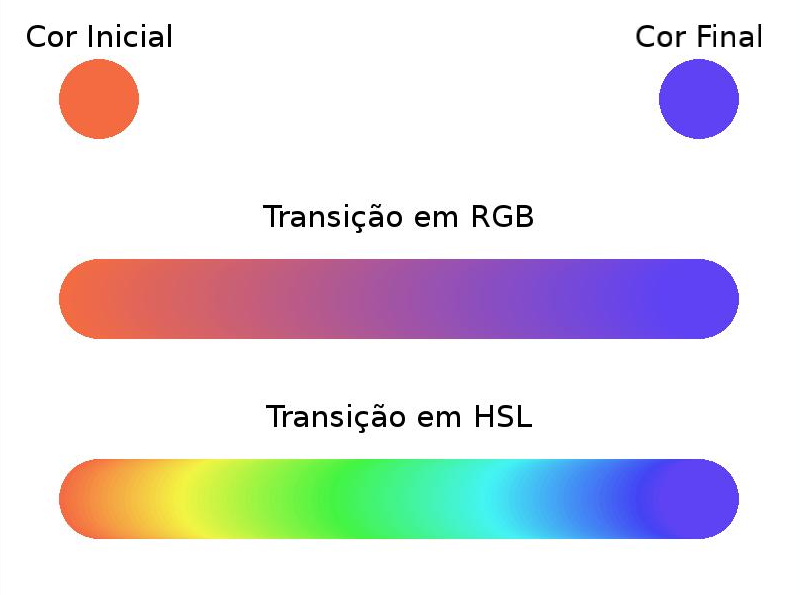
\includegraphics[scale=.3]{color_transitions}
\centering
\caption{Diferença visual de transições usando representação RGB e HSL}
\end{figure}

Com essa mudança, o jogo ficou com transições entre cores muito mais naturais e visualmente belas, se encaixando melhor na temática psicodélica.

A utilização de HSL foi bem direta no programa. Em todos lugares que se tratava de cor, foi utilizado diretamente valores HSL. Somente na hora de desenhar objetos na tela que se faz a transição do valor HSL para RGB (representação utilizada pela função de definir cores no arcabouço \textit{LÖVE}).

A função de converter valores HSL (com todos valores normalizados entre 0 e 255) para RGB é bem simples, baseada na própria geração de cores de RGB para HSL:

\begin{lstlisting}[language={[5.0]lua}]
--Recebe valores de 'h', 's', 'l' (todos no intervalo [0,255]) e retorna
--valores correspondentes de 'r', 'g' e 'b' (tambem no intervalo [0,255]).
function convertHSLtoRGB(h, s, l)
	if s<=0 then return l,l,l end

	h, s, l = h/256*6, s/255, l/255

	local c = (1-math.abs(2*l-1))*s
	local x = (1-math.abs(h%2-1))*c
	local m,r,g,b = (l-.5*c), 0,0,0

	if h < 1     then
		r,g,b = c,x,0
	elseif h < 2 then
	 	r,g,b = x,c,0
	elseif h < 3 then
	 	r,g,b = 0,c,x
	elseif h < 4 then
	 	r,g,b = 0,x,c
	elseif h < 5 then
	 	r,g,b = x,0,c
	else
	 	r,g,b = c,0,x
	end

	return (r+m)*255,(g+m)*255,(b+m)*255
end
\end{lstlisting}

Por último, como nossa função recebe valores nos intervalos [0,255] e normalmente a matiz, saturação e luminosidade são dadas em graus, porcentagem e porcentagem respectivamente, foi criado uma função que faz essa transformação:

\begin{lstlisting}[language={[5.0]lua}]
--Converte os valores HSL em [graus, porcentagem, porcentagem)
--para o intervalo [0-255]
function HSLtoStandardValues(h,s,l)
  local sh = h*255/360
  local ss = s*255/100
  local sl = l*255/100
  return sh, ss, sl
end
\end{lstlisting}
